\chapter{Simulação} \label{cap:simulacao}
\vspace{-2cm}

Este capítulo será apresentada a plataforma \ac{Geant4}, interface usada para simulação de eventos ocorridos no experimento $\nu$-Angra, e as medidas e métodos de simulação realizados neste trabalho \cite{geant4doc}.

\section{Geant4}

Geant4 é um software de código livre, extensível,  utilizado para simular de forma acurada a passagem de partículas por matéria. Todo o escopo de simulação está incluso nas ferramentas do simulador, como construção do detector, materiais, partículas de interesse.

Já incluso no cerne do simulador estão vários modelos físicos para lidar com as interações das partículas por todo uma extensão de níveis energéticos. Construído com uma linguagem orientada à objetos (C++), ele utiliza o método de Monte-Carlo para cálculos, utilizando de métodos estocásticos para resolver as interações determinísticas, do ponto de vista do simulador.

\begin{figure}[H]
	\centering
	
\includegraphics[width=3cm]{textuais/simulacao/figuras/g4.png}
	\caption{Logo do Geant4}
	\label{fig:logo}
\end{figure}

Devido à sua extensibilidade e confiabilidade, o Geant4 foi escolhido como plataforma de simulação para o experimento.
Além de ser utilizado como simulador na física de altas energias, o Geant 4 também possui campo de aplicação em áreas como medicina, para simular tratamentos com radiação; a física nuclear; e as aplicações espaciais, para estudar as interações entre os raios cósmicos e os equipamentos utilizados por astronautas.

\subsection{Construção do detector e parâmetros do experimento}

Valendo-se da plataforma \textit{Geant4}, a Colaboração Neutrinos Angra criou um modelo do detector completo, porém este não considerava mudanças recentes ocorridas no em seu processo de montagem. Portanto, uma das primeiras tarefas relacionadas a este trabalho foi a atualização do modelo do detector no \textit{Geant4} obtendo a forma final apresentada na Figura \ref{fig:detector}. Estes ajustas foram adicionados ao pacote da Colaboração de modo que todos pudessem usar a geometria correta do detector em suas simulações. 

\begin{figure}[H]
	\centering
	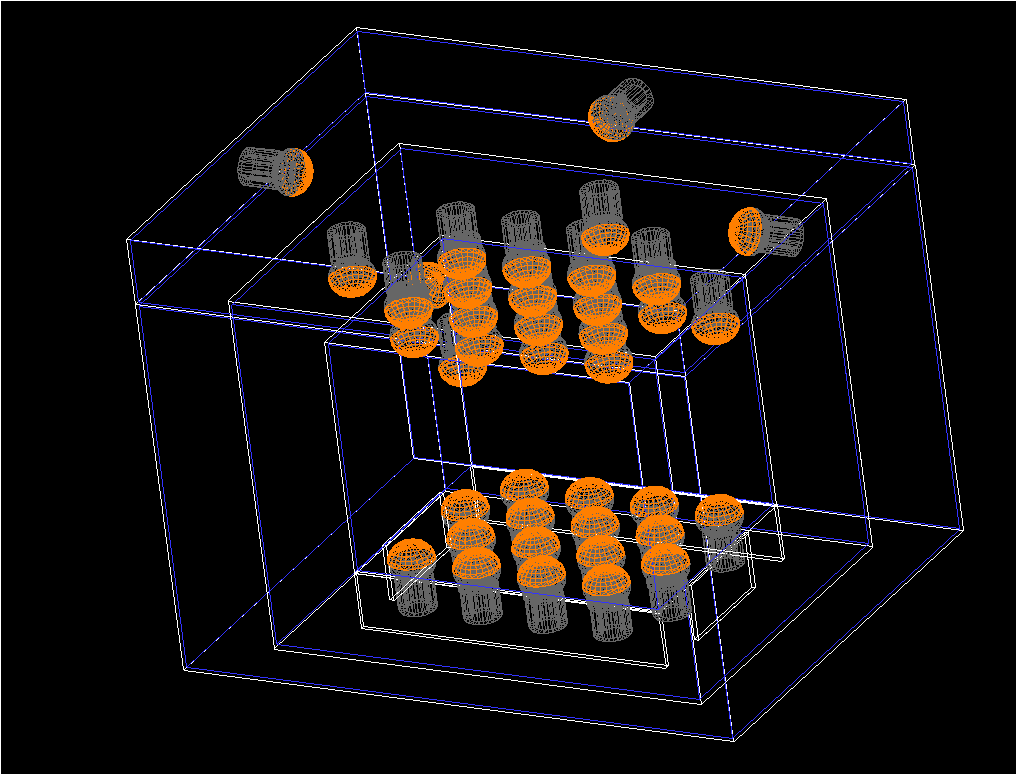
\includegraphics[width=10cm]{textuais/simulacao/figuras/sim_det.png}
	\caption{Detector visto pelo Geant4}
	\label{fig:simdetector}
\end{figure}

A lista de física utilizada foi \emph{QGSP\_BIC\_HP}, que contém os modelos:



\begin{table}[H]
	\centering
	\begin{tabular}{|c|c|c|ll}
		\cline{1-3}
		Sigla & Nome do modelo               & Nível de energia        &  &  \\ \cline{1-3}
		QGS   & Quark Gluon String model     & \textgreater 12 GeV     &  &  \\ \cline{1-3}
		FTF   & FRITIOF String model         & 9.5 - 25 GeV            &  &  \\ \cline{1-3}
		BIC   & Binary Cascade model         & 200 MeV - 9.9 GeV       &  &  \\ \cline{1-3}
		HP    & High Precision neutron model & \textless{}$\sim$20 MeV &  &  \\ \cline{1-3}
	\end{tabular}
	\caption{Modelos de física utilizados}
\end{table}

Estes modelos foram escolhidas devido às interações de interesse na simulação, sendo a interação de raios cósmicos com o detector, que variam entre $100$ MeV e $10$ GeV.


\section{Geração das partículas}

As partículas de simulação foram geradas pela plataforma ROOT, da colaboração do \ac{CERN}, para realizar os cálculos. Para facilitar a simulação dos eventos, ao invés de implementar as pás no simulador, os raios cósmicos são gerados já passando por elas, garantindo o \emph{trigger} do sistema para qualquer evento da lista. 

 Na geração das partículas foi utilizado um modelo aleatório de sorteio em histogramas com as distribuições das direções nos eixos $x$,$y$ e $z$ e a posição inicial no plano 3D \cite{amarogithub}, depois foi calculado em que posição estará a partícula na altura das duas pás e, se ela estiver dentro da área de ambos, salva a partícula. Uma pequena amostragem dos eventos salvos podem ser vistos na Figura \ref{fig:geracao}.

\begin{figure}[H]
	\centering
	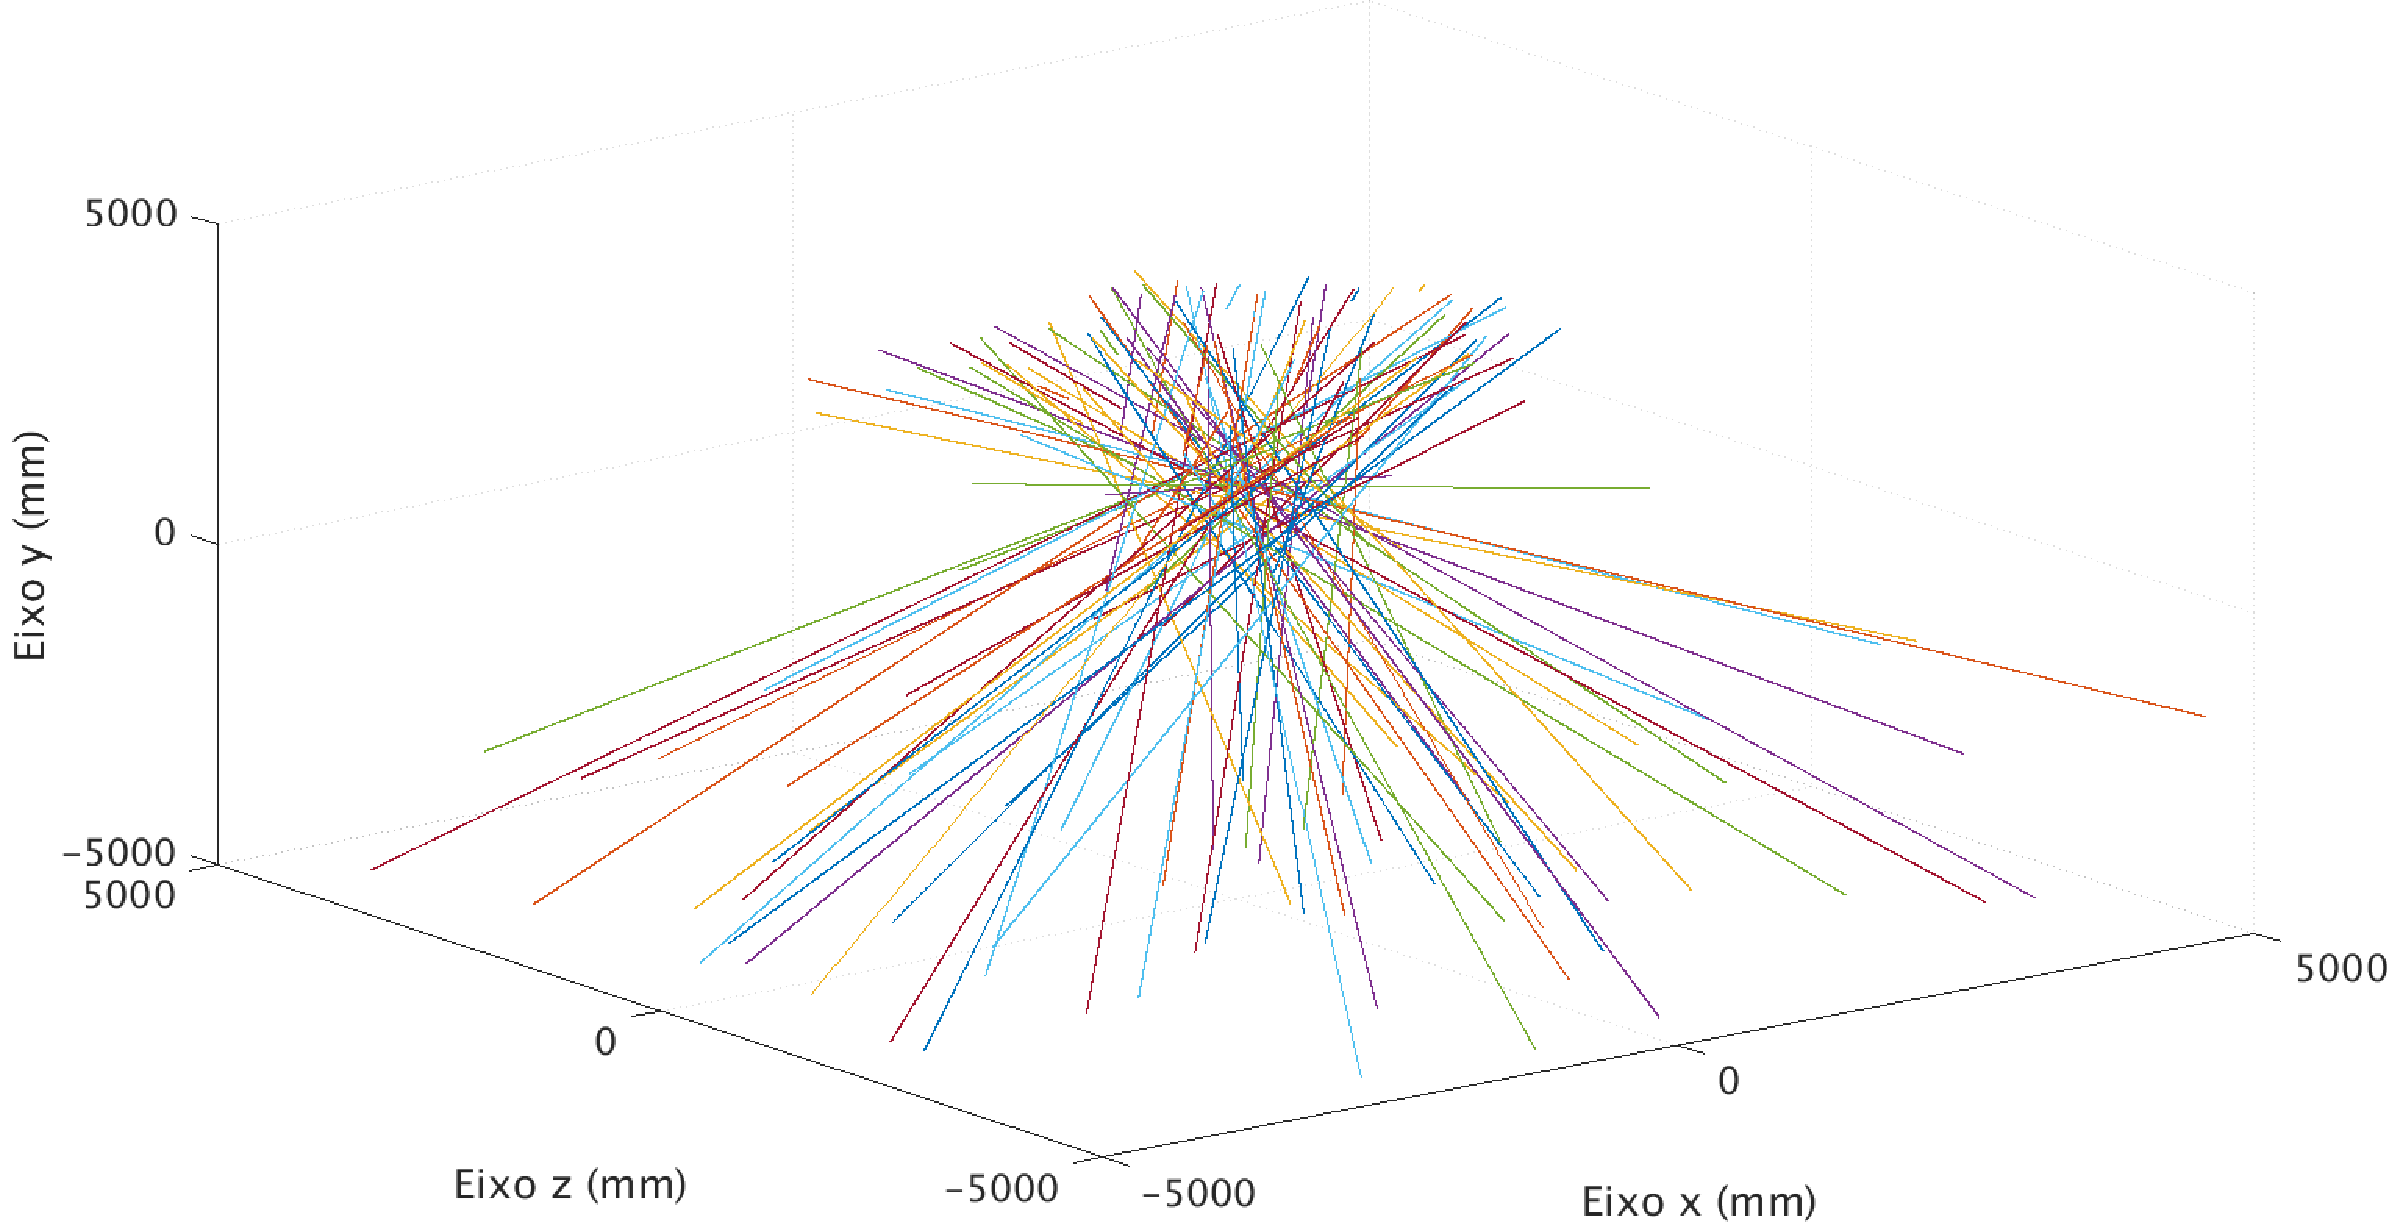
\includegraphics[width=14cm]{textuais/simulacao/figuras/geracao.pdf}
	\caption{Raios cósmicos gerados}
	\label{fig:geracao}
\end{figure}


\section{Simulação inicial}

Assim, com o \emph{Geant4} configurado e as partículas geradas podemos executar a simulação e fazer a análise dos resultados. Foram realizadas a simulação de $20000$ eventos. As Figuras \ref{fig:a} e \ref{fig:b} mostram uma comparação entre os dados reais e simulados do espectro de energia dos eventos e da distribuição da energia deixada nas PMTs.

\begin{figure*}[ht]
	\centering
	\begin{subfigure}{0.5\textwidth}
		\centering
	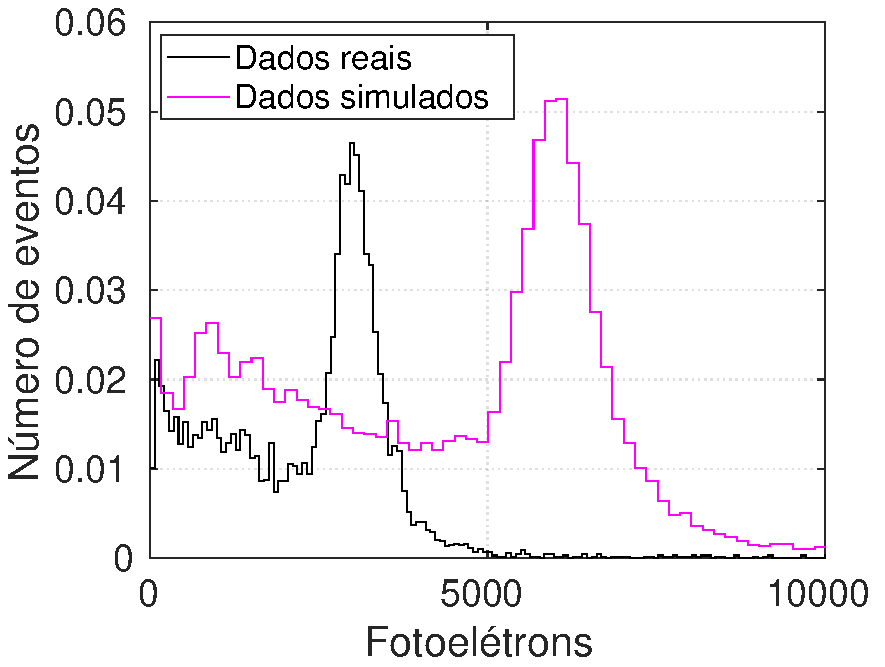
\includegraphics[width=8cm]{textuais/simulacao/figuras/hist_pmt1.pdf}
		\caption{Distribuição de p.e. por eventos}
		\label{fig:a}
	\end{subfigure}%
	~ 
	\begin{subfigure}{0.5\textwidth}
		\centering
	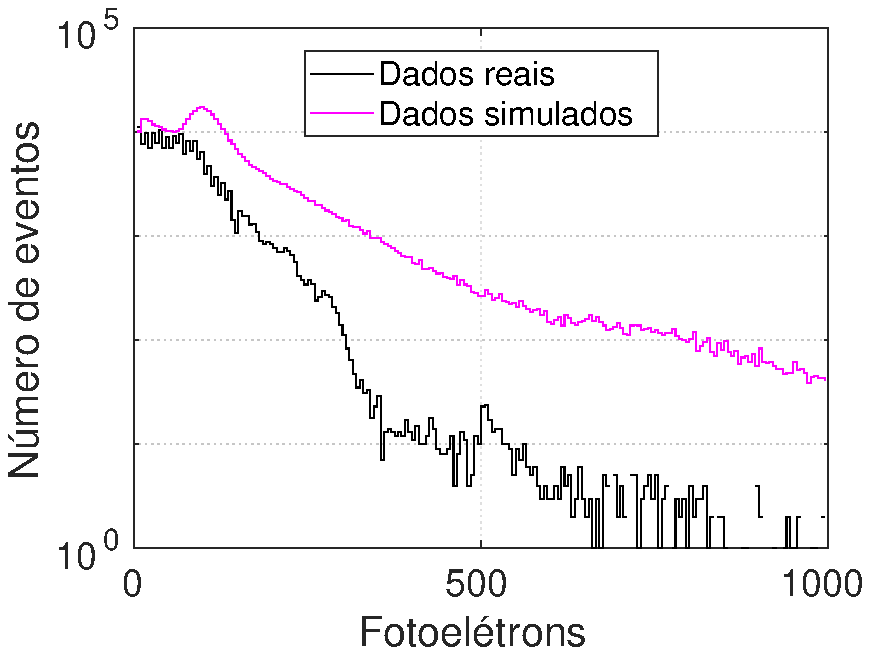
\includegraphics[width=8cm]{textuais/simulacao/figuras/hist_evt1.pdf}
		\caption{Distribuição de p.e. por PMT}
				\label{fig:b}
	\end{subfigure}
	\caption{Comparação dos dados reais com os simulados.}
\end{figure*}

Outros plots podem ser encontrados no apêndice \ref{apdx:simantesantes}.

\section{Propostas de ajuste para casar dados reais com dados simulados} \label{sec:bugs}

Como pode ser percebido, há um erro de calibração do sistema simulado, de forma geral os eventos apresentam muito mais energia  do que no sistema real, então, muito mais fotoelétrons estão sendo capturados pelas PMTs. Algum método deve ser encontrado para calibrar a simulação. A partir deste ponto, como estratégia, iremos considerar que os ajustem devem ocorrer na simulação e não o contrário. Em alguns casos ajustes poderiam ser aplicados aos dados reais a fim de se mitigar alguns fenômenos como, por exemplo, o efeito da saturação das PMTs que ocorrem quando uma grande quantidade de fotoelétrons são gerados em uma única PMT ou erros no processo de \textit{fitting} quando aplicados na recuperação da forma de onda dos sinais saturados na \textit{front-end}.

\subsection{Correção das PMTs}

O primeiro problema encontrado foi para múons que passam por dentro de PMTs, que geram fótons dentro da mesma, porém no volume interior da PMT real há vácuo, então não deveria ocorrer a radiação de Cherenkov, dada a energia gerada dentro da PMT pode-se inferir que para a simulação havia água dentro delas. Então foi-se adicionado um volume com vácuo dentro da PMT para corrigir este problema

\begin{table}[H]
	\centering
	\begin{tabular}{|c|c|}
		\hline
		Antes da correção  & 929 eventos \\ \hline
		Depois da correção & 22  eventos \\ \hline
	\end{tabular}

\caption{Número de fotoelétrons gerados por uma PMT do detector devido a passagem de um múon de alta energia por seu interior. Estes valores foram obtidos fazendo passar um múon de alta energia por dento da PMT, antes e depois de se aplicar a correção.}
\end{table}


\subsection{Transformação de CDFe}
\label{CDFe}

Além da qualidade da água, temos que implementar na a simulação a saturação da eletrônica de \emph{front-end} e a não linearidade das PMTs. Foi feita então uma transformação de \ac{CDFe} dos eventos simulados para os dados reais, transformando o histograma de p.e. por PMT dos dados simulados no histograma de p.e. por PMT dos dados reais. Efetivamente modelando diretamente pela distribuição fornecida pelos dados reais.


\begin{figure*}[ht]
	\centering
	\begin{subfigure}{0.5\textwidth}
		\centering
		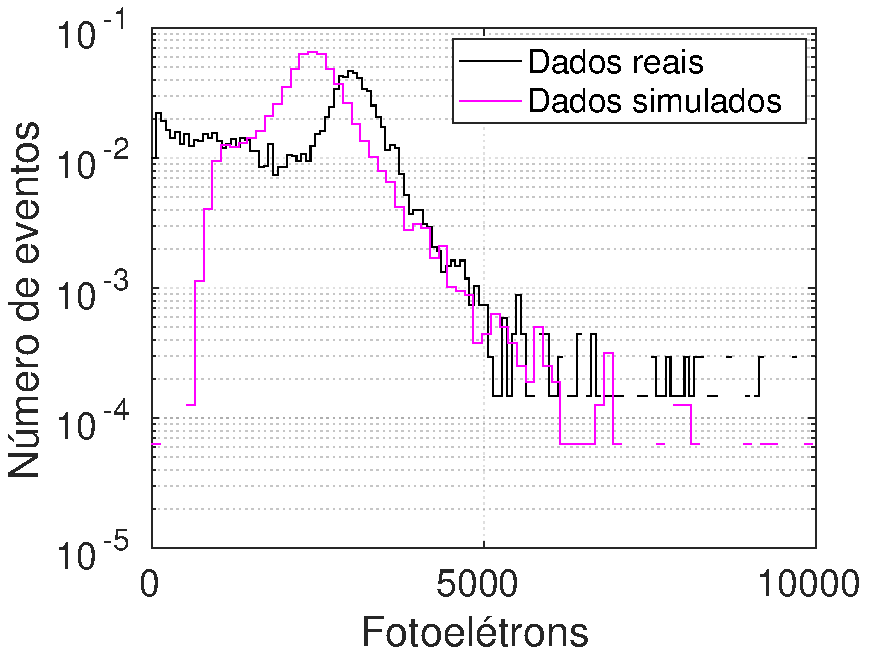
\includegraphics[width=8cm]{textuais/simulacao/figuras/hist_pmt2.pdf}
		\caption{Histograma de p.e. por eventos}
		\label{fig:a2}
	\end{subfigure}%
	~ 
	\begin{subfigure}{0.5\textwidth}
		\centering
		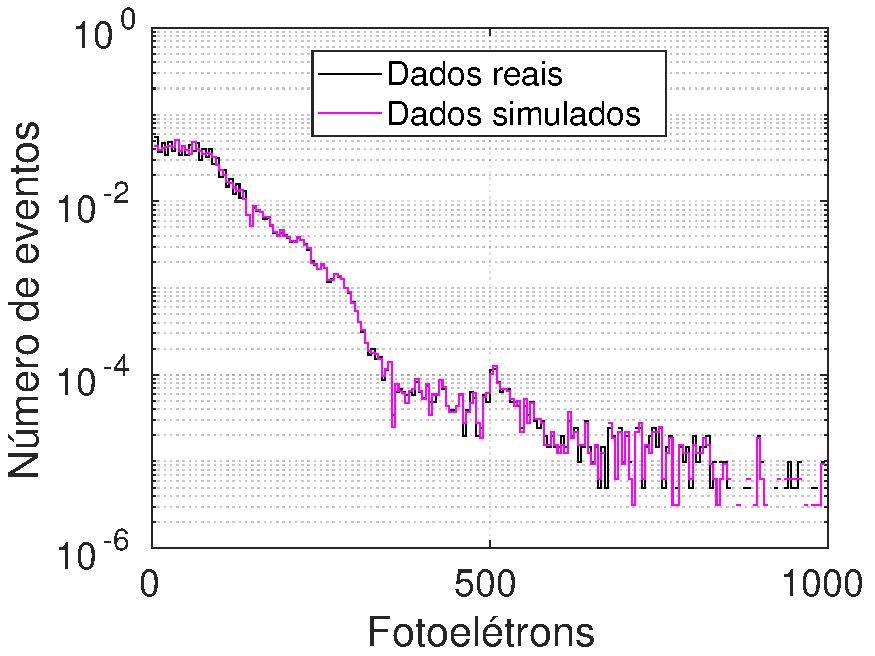
\includegraphics[width=8cm]{textuais/simulacao/figuras/hist_evt2.pdf}
		\caption{Histograma de p.e. por PMT}
		\label{fig:b2}
	\end{subfigure}
	\caption{Comparação dos dados reais por simulados após a transformação de CDFe}
\end{figure*}

Como era de se esperar, a transformação de CDFe resolveu o problema que o histograma de p.e. por PMT apresentava, porém o problema por eventos apenas se agravou. As PMTs com pouco número de p.e. detectados foram substituídos por um número maior de p.e. devido à falta de dados na simulação para baixas energias, transformando um número pequeno de p.e. em um número maior. Para contornar este problema de baixas energias após o método da CDFe, serão transformados apenas os valores de PMTs que estão além do ponto de saturação, utilizado neste trabalho $200$ p.e. como parâmetro, resultando na Figura \ref{fig:cdfe}.

\begin{figure}[H]
	\centering
	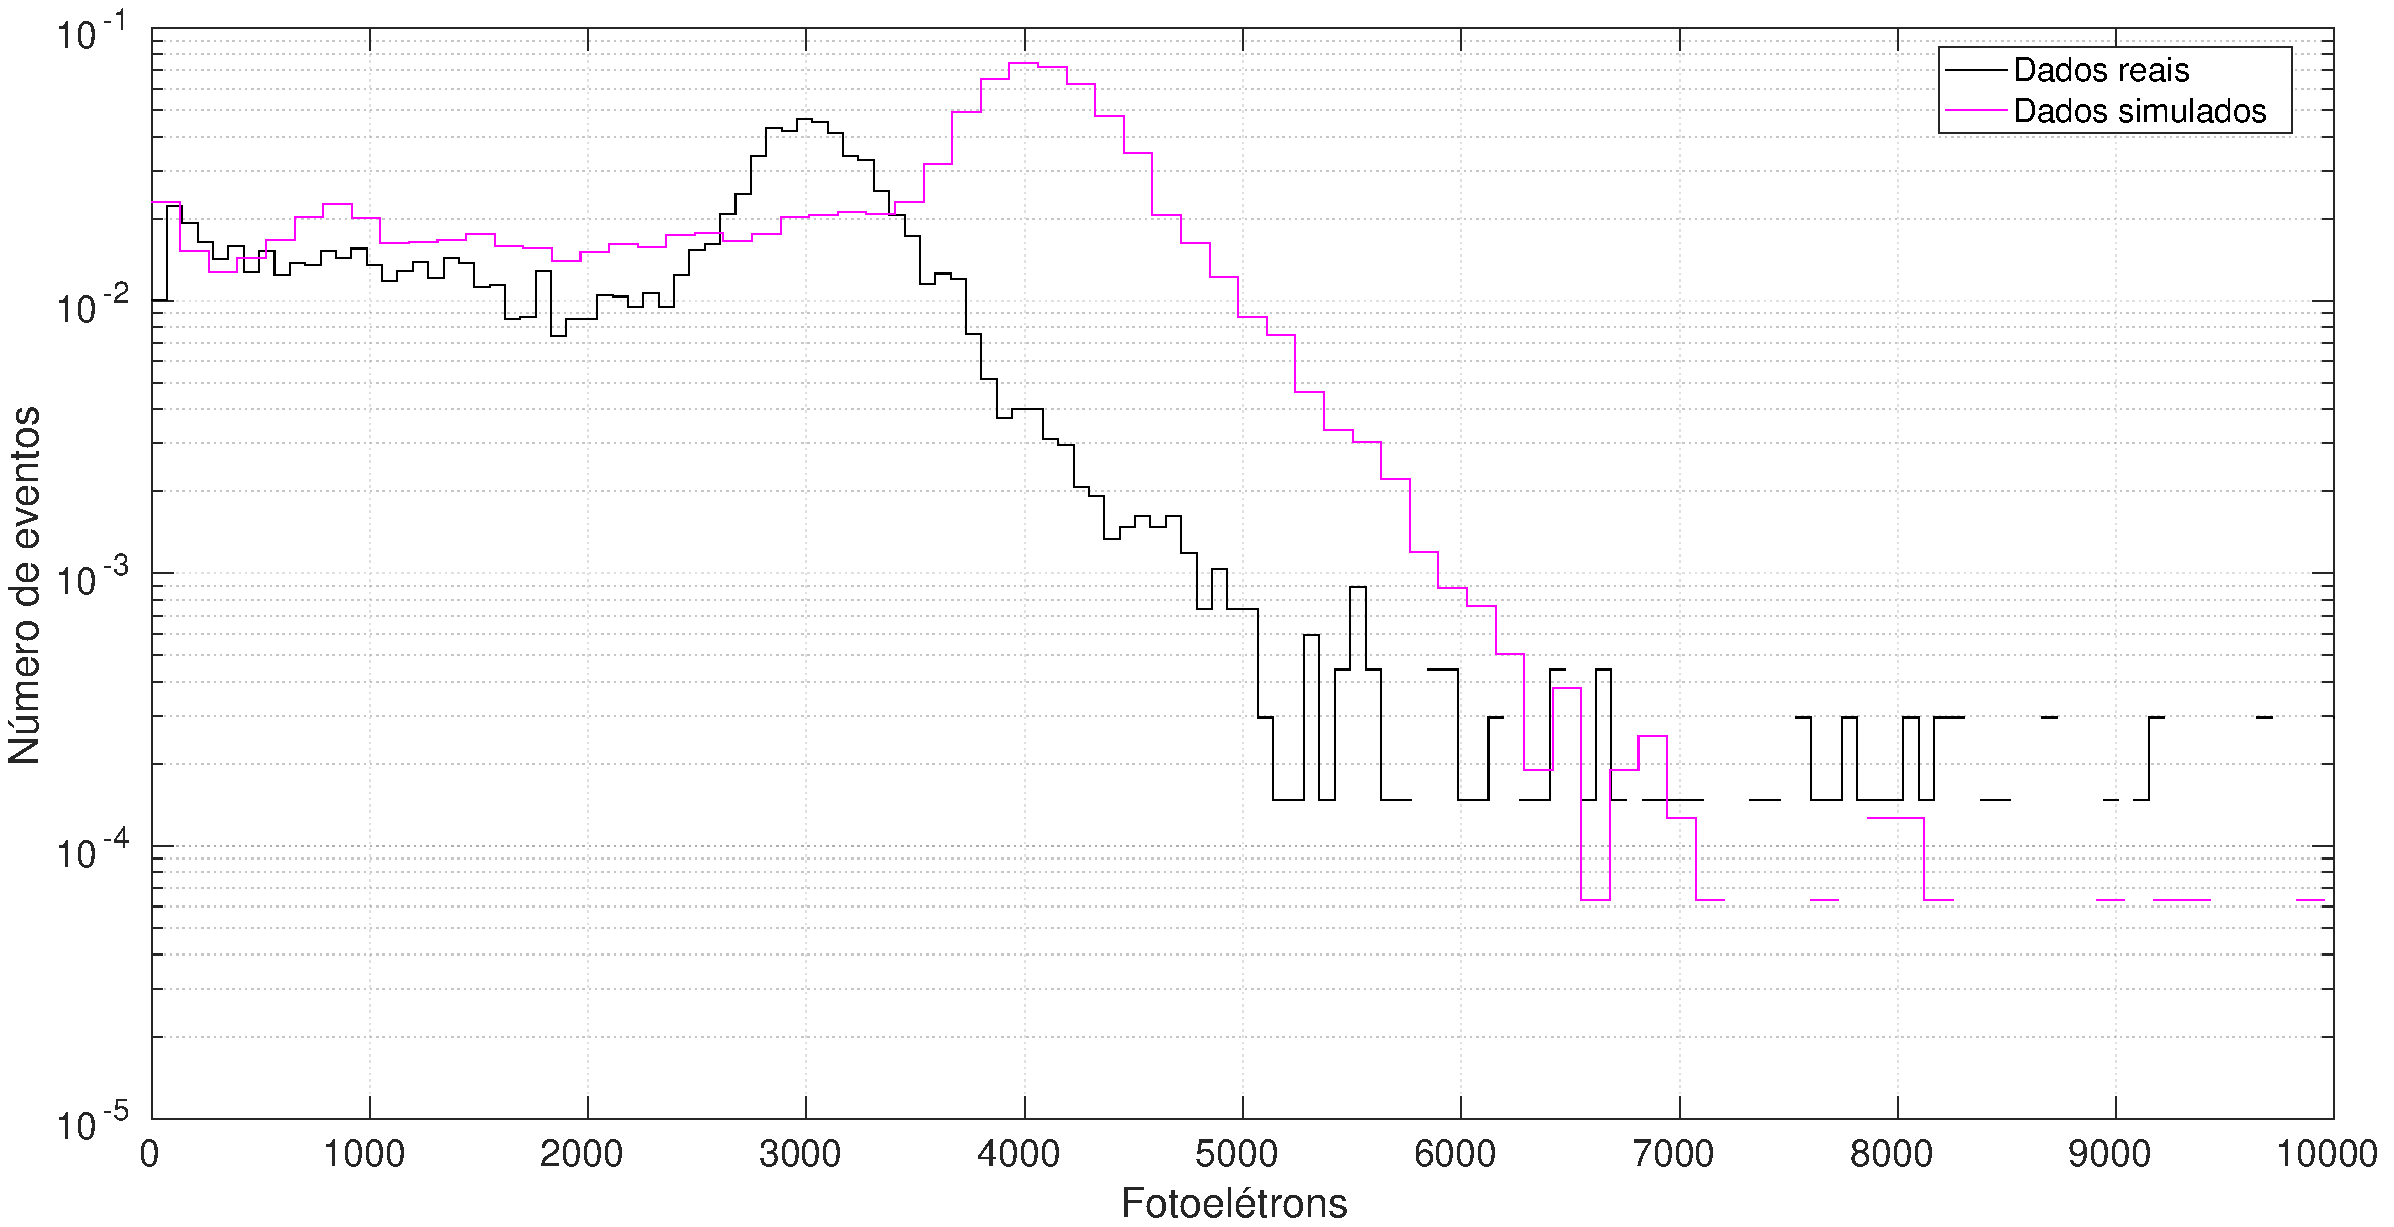
\includegraphics[width=12cm]{textuais/simulacao/figuras/hist_evt6.pdf}
	\caption{Histograma de p.e. por eventos após a CDFe a partir do ponto de saturação}
	\label{fig:cdfe}
\end{figure}

\subsection{Qualidade da água}

Como discutido no Capítulo \ref{cap:experimento} na Sessão \ref{sec:detector}, na água dopada com sal de gadolínio há uma diminuição no caminho médio livre e, na simulação, não há este sistema implementado, sendo utilizado o caminho médio livre de uma água completamente pura. Além disto, a qualidade da água em Angra nunca foi medida de fato, podendo não corresponde aos parâmetros referentes utilizados na simulação. Então deve-se alterar a qualidade da água para que a distribuição de energia produzida pela simulação se aproxime daquela produzida pelos dados reais.

Para tal, utilizaremos um modelo iterativo diminuindo o caminho médio livre do fóton na água e ajustando o número de p.e. gerados nas PMTs (seção \ref{CDFe}) até que os dados simulados representem os dados reais. As Figuras \ref{fig:a3} e \ref{fig:a4} a seguir mostram alguns passos deste processo iterativo.



\begin{figure*}[ht]
	\centering
	\begin{subfigure}{0.5\textwidth}
		\centering
		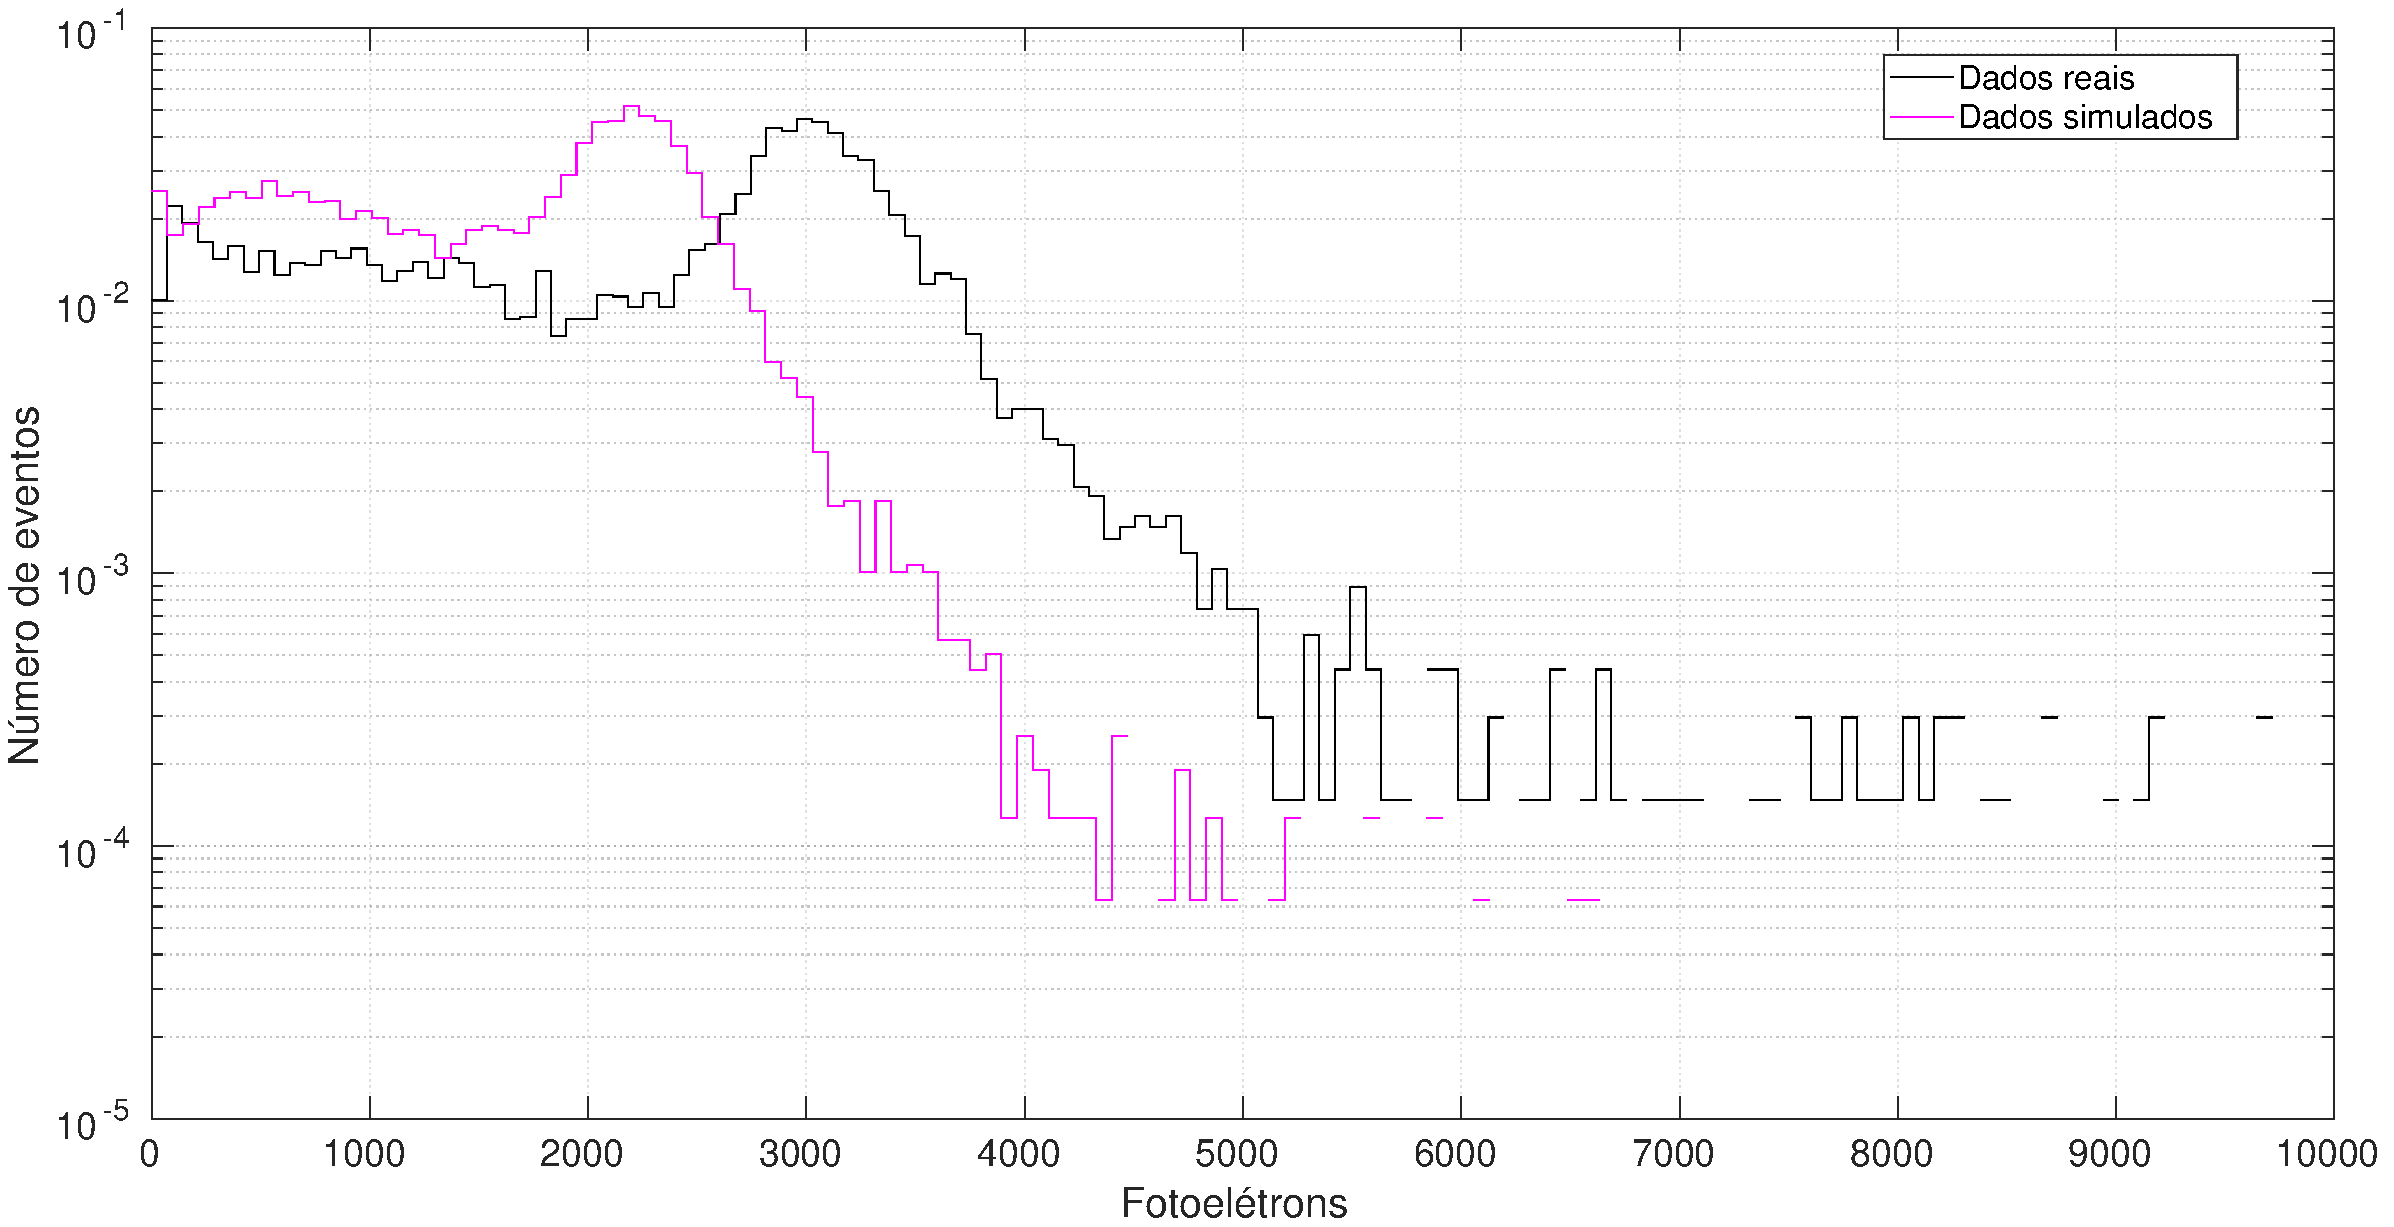
\includegraphics[width=8cm]{textuais/simulacao/figuras/hist_evt3.pdf}
		\caption{Qualidade da água 86\% pior que a original}
		\label{fig:a3}
	\end{subfigure}%
	~ 
	\begin{subfigure}{0.5\textwidth}
		\centering		
		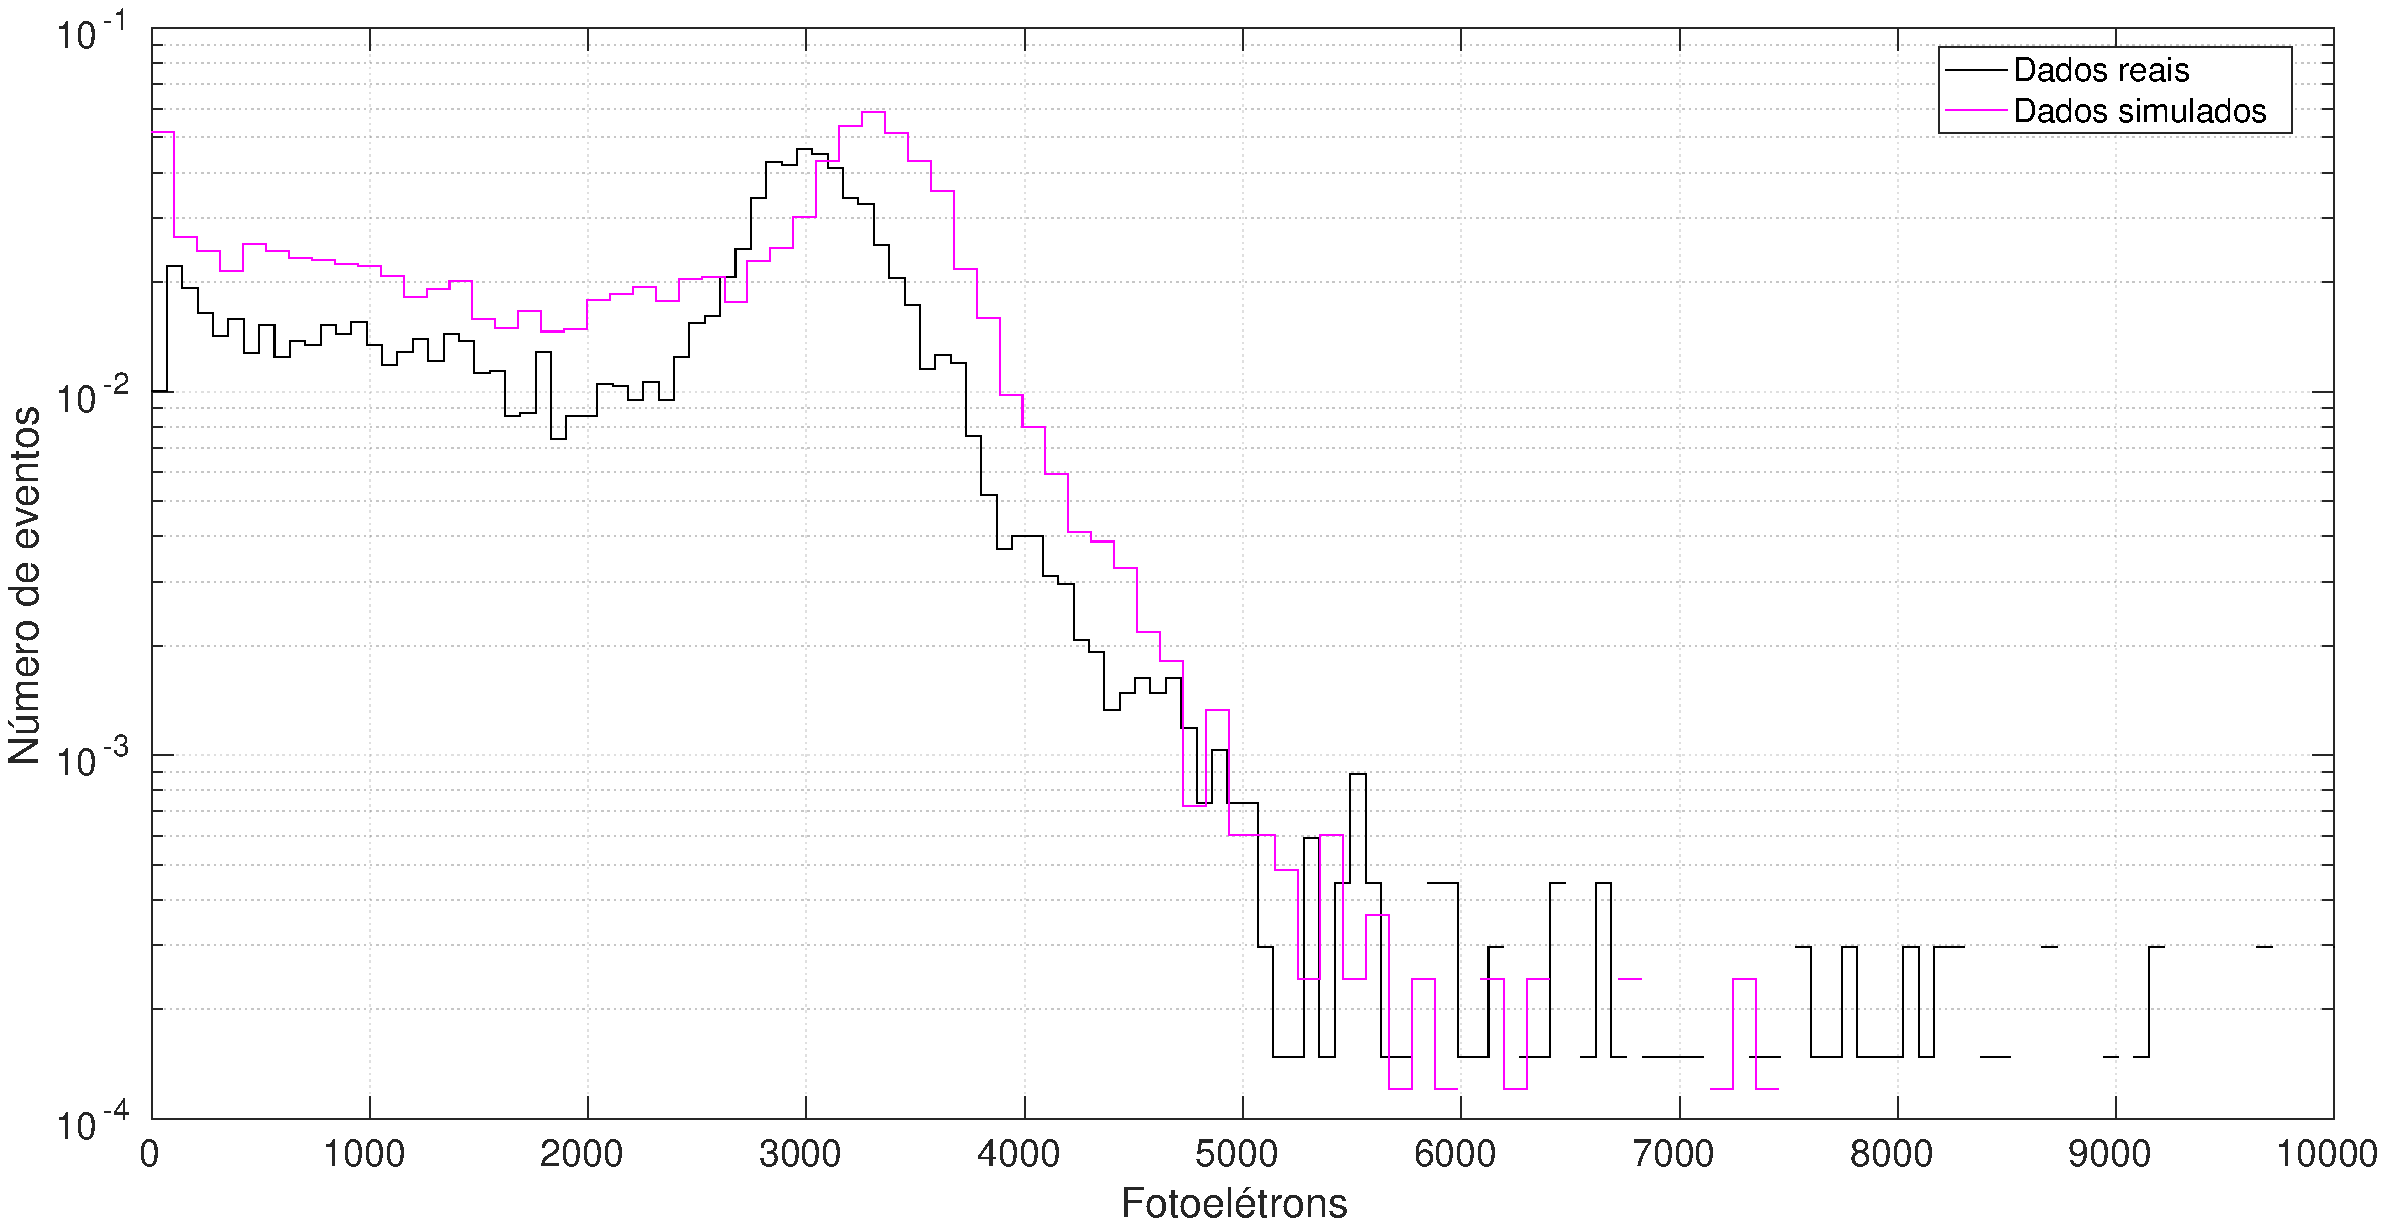
\includegraphics[width=8cm]{textuais/simulacao/figuras/hist_evt5.pdf}
		\caption{Qualidade da água 75\% pior que a original}
		\label{fig:a4}
	\end{subfigure}
	\caption{Comparação dos dados reais por simulados após a transformação de CDFe modificando a qualidade da água}
\end{figure*}

Como se utilizou de um método iterativo e intuitivo, não foram necessárias mais do que quatro iterações para encontrar o valor da qualidade da água utilizado. Porém a projeção do erro entre a distância dos picos para a água pode ser visto na Figura \ref{fig:erro_qualidade}. Onde o eixo $x$ representa a qualidade da água em porcentagem, enquanto o eixo $y$ representa o erro entre as distâncias dos picos.

\begin{figure}[H]
	\centering
	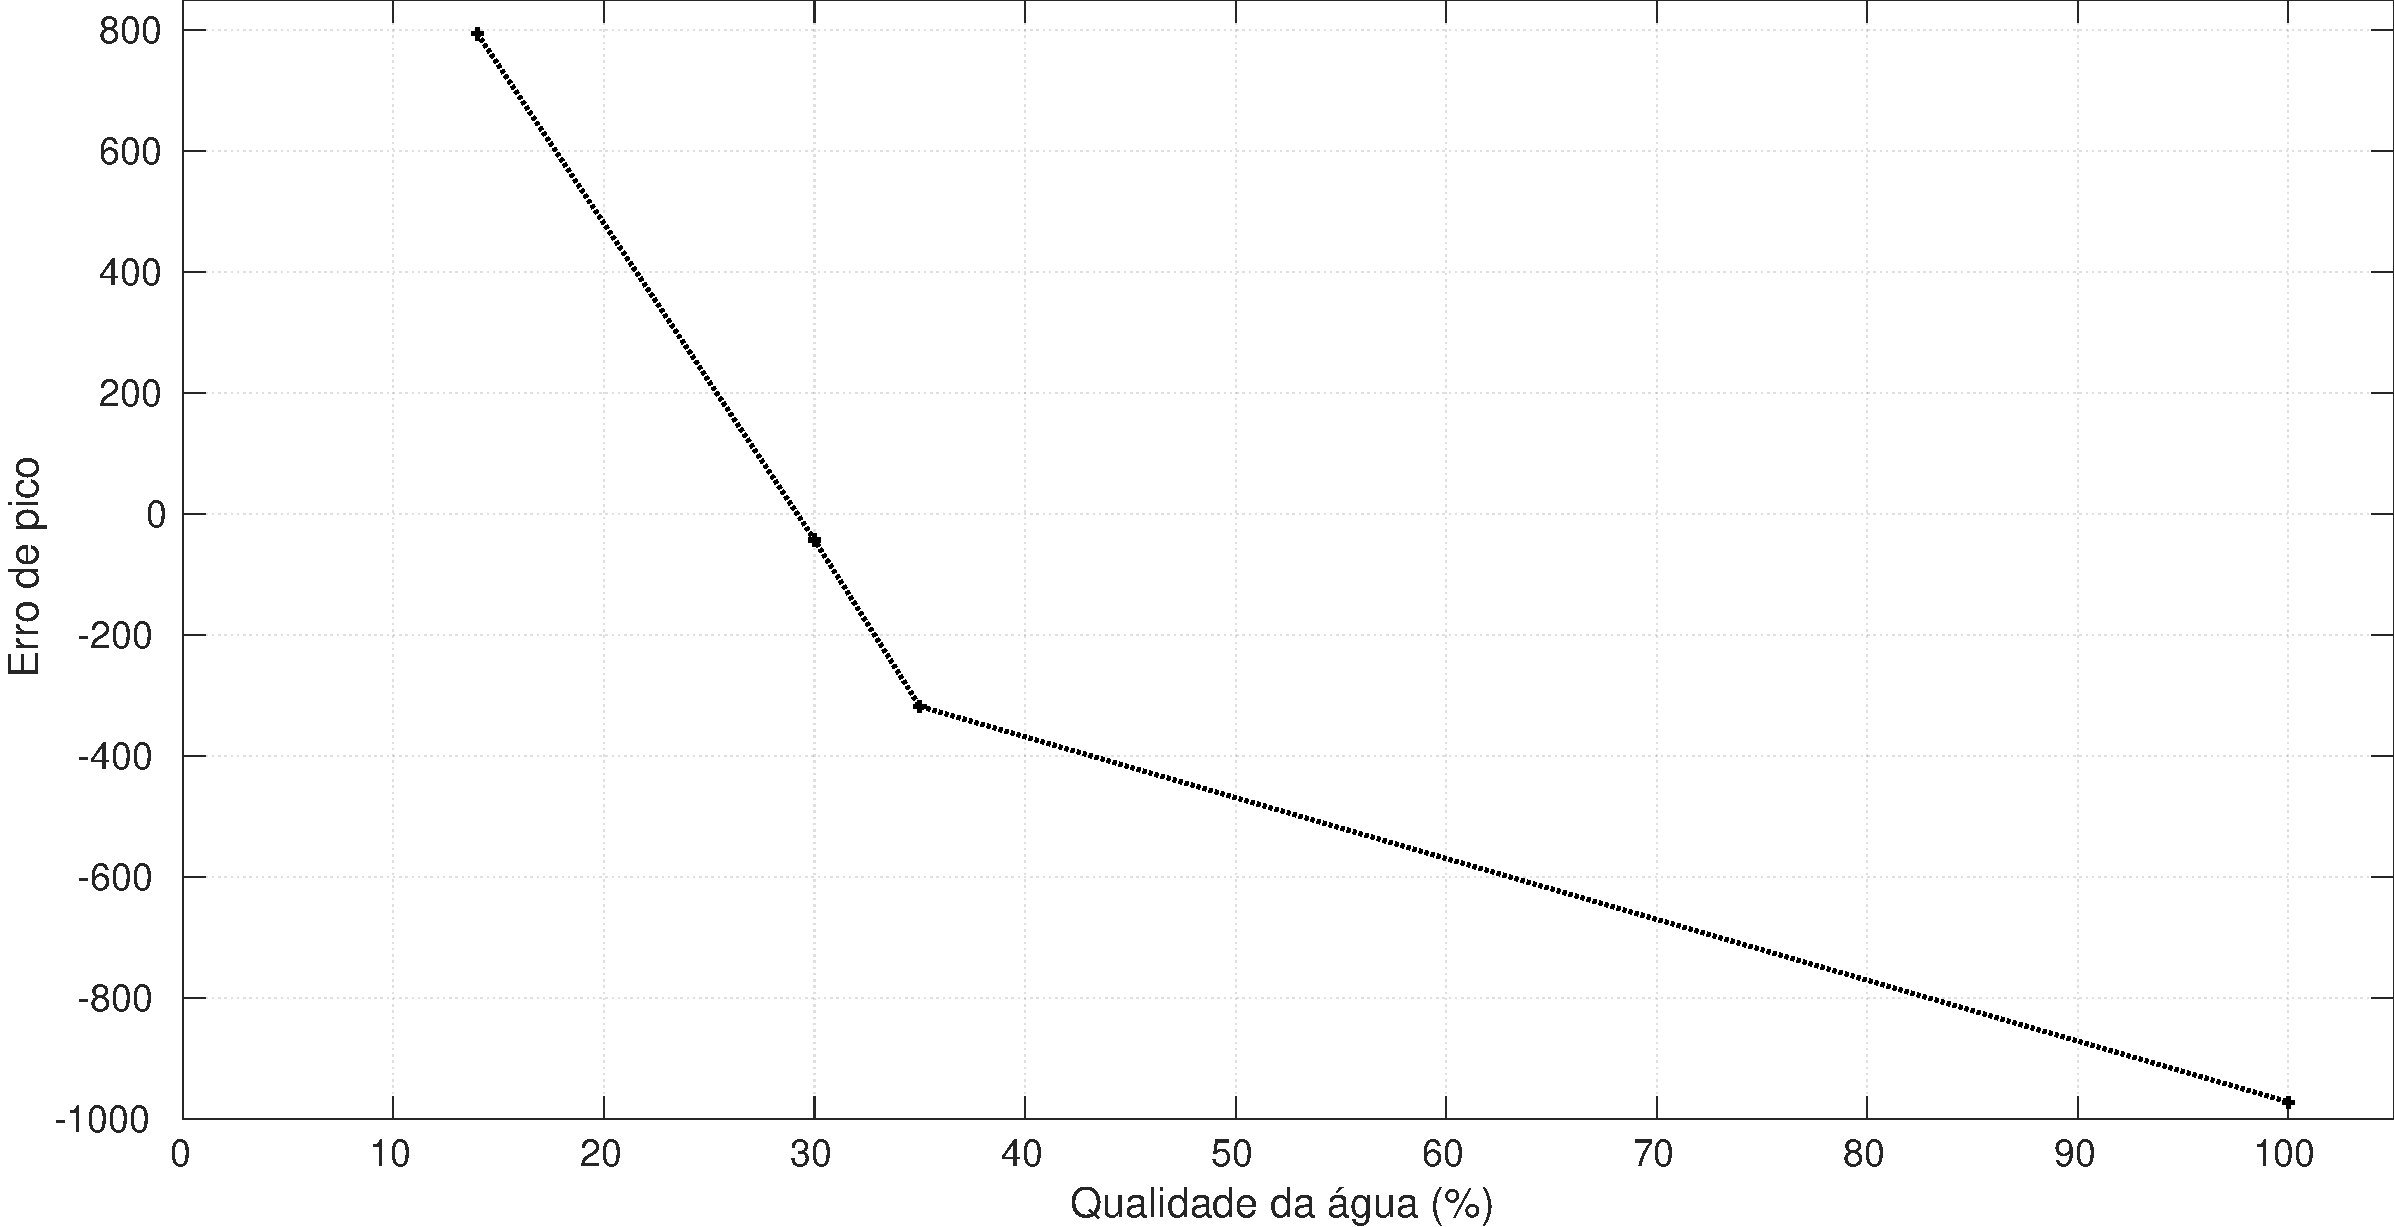
\includegraphics[width=16cm]{textuais/dadosreais/figuras/erro_qualidade.pdf}
	\caption{Erro das distâncias dos picos de energias versus qualidade da água }
	\label{fig:erro_qualidade}
\end{figure}
